
\chapter{Design in reaction to CDCS}

From its very inception, Skedge's functionality and visual design were driven by the shortcomings of CDCS. Skedge is built \emph{bottom-up}, not \emph{top-down}---every aspect of the application was either made as a reaction to a particular grievance in CDCS or as the natural evolution of an existing feature. Skedge is thus rooted in \emph{usability} derived from real need, not mere conjecture along the question ``what could students want?''. Its success with students, shown in Chapter 4, demonstrates that this usability extends beyond my own standard and can fulfill the various discovered use-cases of students in general.

In this chapter, I invite the reader along on a tour of these grievances and their remedies.

%%%

\section{Modernity}

CDCS is an old system, relatively speaking, and its development on user-facing features has been almost entirely stagnant. It launched in 2009, seven years ago, and has hardly changed since. Figure \ref{fig:cdcs2010} shows CDCS in July 2010, which, besides the addition of a few search fields, is identical to its current version. Yet, since its introduction in 2009, we have seen the rise of mobile devices into ubiquity, a boom in ``hacker culture'' and public APIs, and the capability for standalone web applications to be as sophisticated and dynamic as desktop-class applications without the aid of browser extensions. With this in mind, Skedge brings course scheduling to the modern era.

\begin{figure}[ht]
  \centering
    \fbox{
      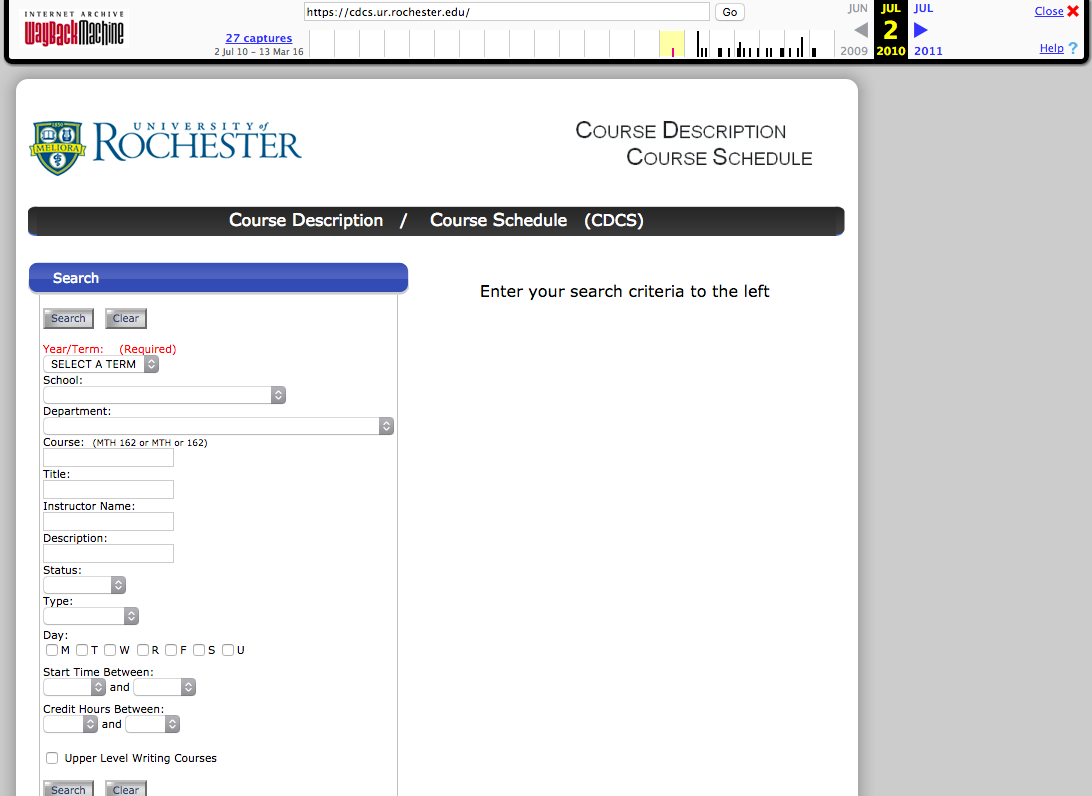
\includegraphics[width=10cm]{images/cdcs/2010}
    }
  \caption{CDCS in July 2, 2010, virtually unchanged from today, courtesy of \emph{Archive.org}}
  \label{fig:cdcs2010}
\end{figure}

\subsection{AJAX vs. GET requests}

CDCS makes an AJAX request with every submitted search, meaning that the server receives the request and returns a response all without any page navigation (i.e. the URL stays the same and no new page is loaded as the search results are displayed). Skedge, however, makes a GET request for every search submission, meaning that the user's browser loads a new page that contains the results and whose URL reflects the search query. This simple technical design decision substantially increases usability for two reasons:

\begin{enumerate}
  \item Page navigations allow users to leverage their browser history as it was designed---after making several searches, CDCS users who use the back button on their browsers will be brought to the page loaded before the very first use of CDCS, possibly losing time spent in crafting sophisticated searches. Skedge users can go backwards and forwards through their search histories and scroll locations using native browser functionality.
  \item Every search query has a unique URL (e.g. \url{http://skedgeur.com/?q=csc} for {\tt csc}), so users are able to send links to a specific course or search result to others. With CDCS, the URL remains \url{https://cdcs.ur.rochester.edu} throughout the duration of the session.
\end{enumerate}


\subsection{Mobile}

According to Mary Meeker's 2015 Mobile Technology Trends from Kleiner Perkins Caufield \& Byers\cite{kpcb}, in 2014, 51\% of adult time spent per day on the Internet was from a mobile device, versus 42\% spent on a desktop computer or laptop. Time spent on the Internet with mobile devices reached three hours per day in 2014, compared to less than one hour in 2010 (12\% mobile vs. 75\% desktop/laptop time share).

Undeniably, supporting mobile devices and tablets in web applications is crucial for usability nowadays. Note how Skedge is responsive to the user's device in Figure \ref{fig:sk-mobile}, compared with CDCS's lack of mobile support in Figure \ref{fig:cdcs-mobile}. CDCS on mobile requires the user to pinch and drag around both to read results and to make new searchs, while Skedge adapts content to the device's screen and fixes the search bar to the top of the screen for easy access while browsing.

Moreover, since no major mobile browser currently supports browser extensions (and if one did, the extensions themselves would most likely need to be re-architected), CDCS on a mobile device loses all scheduling functionality, unlike with Skedge on mobile.

\begin{figure}[ht]
  \centering
  \vspace{10pt}
  \begin{tabular}{c c}
    \begin{subfigure}[h]{4.5cm}
      \centering
      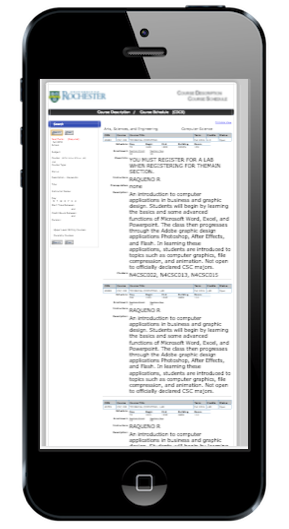
\includegraphics[width=1.00\textwidth]{images/cdcs/mobile}
      \caption{CDCS} \label{fig:cdcs-mobile}
    \end{subfigure}
    \begin{subfigure}[h]{4.4cm}
      \centering
      
\includegraphics[width=1.00\textwidth]{images/skedge/mobile}
      \caption{Skedge} \label{fig:sk-mobile}
    \end{subfigure}
  \end{tabular}
  \caption{CDCS and Skedge running on a mobile device}
\end{figure}

\subsection{Public API}

With the increasing number of attendees at University of Rochester's hackathons, it is clear that the University's ``hacker culture'' is growing---more students are collaborating to build side-projects that integrate resources and servies often benefitting the student community. Open-source and open-information services greatly help to foster such innovation, and having public APIs is essential toward this end.

Skedge provides a public JSON API at the root URL \url{http://www.skedgeur.com/api/}, made at the request of a student that was interested in using its course data, and the API has already been used in projects by several other student groups. The endpoints included are \url{/api/courses?q=query} (Skedge's query language---described in detail in section 2.3---is supported here), \url{/api/departments?q=optional_query}, and \url{/api/instructors?q=optional_query}.

\subsection{Built-in scheduler}

As explained in the introduction, Skedge offers users a course schedule right in the page, unlike CDCS which requires the Better CDCS browser extension for this functionality. Having a schedule native in the application has several advantages:

\begin{enumerate}
\item Besides some CDCS users possibly not even knowing about Better CDCS, not requiring a browser extension provides for a faster and more seamless user onboarding, especially when building schedules on public computers when extensions can't always be installed.

\item Skedge accommodates a schedule into its design, whereas Better CDCS has to work around an interface that wasn't designed with one. As a result, Better CDCS has lower usability, requiring the user to toggle between search results and their schedule. Skedge, conversely, gives users immediate visual feedback on how a course would fit into their schedule.

\item Schedule data is centralized on Skedge's servers as opposed to locally in a browser cache, meaning that it can synchronize across a user's devices or in sessions on public computers, persists browser resets, and can be easily publicly shared to other users.

\item Extensions like Better CDCS have limited browser support. Internet Explorer and mobile browsers are unsupported, for example.
\end{enumerate}

%%%

\section{Usability}

\subsection{Visual presentation}

Skedge offers several improvements over CDCS in the quality of its data presentation:

\begin{enumerate}
  \item Displaying information in a rigid, tabular way, CDCS does not leverage fonts and styling to adhere to typographical standards. Instead of using larger or bolder type, for instance, course titles are listed entirely in uppercase (e.g. ``INTRO TO PROGRAMMING''), which has been shown to be less readable than lower-case text \cite{caps}. This problem is compounded when users browse through possibly hundreds of courses. Skedge displays properly capitalized titles styled with large type that helps users to quickly group and locate them.

  \item While possibly not a fault of the CDCS system itself, there are very frequently typos or missing spaces in the ``comments'' section of courses, which Skedge corrects.

  \item CDCS displays all course times in 24-hour time, which, despite being concise and unambiguous, is not what most US students are used to. Skedge displays 12-hour time with AM/PM, and prevents ambiguities through the course-in-schedule visualization on hover.
\end{enumerate}

\subsection{Section display}

Often, courses are offered at multiple timeslots, sometimes taught by different instructors and in different rooms. These are called \emph{sections} of a course. CDCS displays each section in a discrete ``section box'' (all of which are nondistinct and have equal size), even if two sections pertain to the same course. (In this regard, CDCS should really be \emph{SDSS}, ``\emph{Section} Description / \emph{Section} Scheduler'', because it operates on the level of sections, not courses.) As a result, course descriptions (which can be lengthy), titles, prerequisites, comments, etc. are all repeated for every section of the course.

To make matters worse, many courses in the University course catalog include what I call \emph{subsections}---secondary sections associated with a course that must be registered for separately. Namely, these are labs, lab lectures, workshops, and recitations. Once again, CDCS displays \emph{all of these} as separate ``section boxes'' by default, and the course description is yet again repeated for each subsection (which, this time can be tens of times), wasting valuable page space.

Collapsing subsections within courses can result in massive improvements in filtering the data most relevant to the user. For instance, the search {\tt csc} for Fall 2016 on CDCS results in 147 ``section boxes'', while Skedge only shows 45 ``\emph{course} boxes'', with subsections collapsed within their respective course. This triage reduces the data (noise, more correctly) displayed by ~70\%, and is even higher for departments with more abundant labs and workshops, such as Physics (Skedge: 35 vs. CDCS: 226, an ~85\% reduction), or Chemistry (Skedge: 25 vs. CDCS: 171, an ~86\% reduction).

Skedge can reduce the amount of data to scroll through---and thus the time taken to do so---by six- or seven-fold (and possibly more, counting the attention users otherwise have to pay to distinguish course from subsections), so this design decision has a large usability payoff.

Additionally, some Physics courses (for instance) follow the ``A / B'' subsection structure, where a student registered for an ``A Section'' (as opposed to the ``B Section'') must also register for an ``A Lab'' and ``A Workshop''. Skedge organizes subsections for these cases to help sort the two out, which get mixed up in CDCS's linear output.

Note that in Figure \ref{fig:cdcs-sections} (CDCS), the first two boxes are sections for the same course, and the next two are labs for that course. Four more lab sections and \emph{twenty} more workshop sessions for that same course follow below the truncated screenshot. Figure \ref{fig:sk-sections} (Skedge) demonstrates how this information can be conveyed more concisely.

\begin{figure}[ht]
  \centering
  \vspace{10pt}
  \begin{tabular}{c c}
    \begin{subfigure}[h]{6cm}
      \centering
      \fbox{
        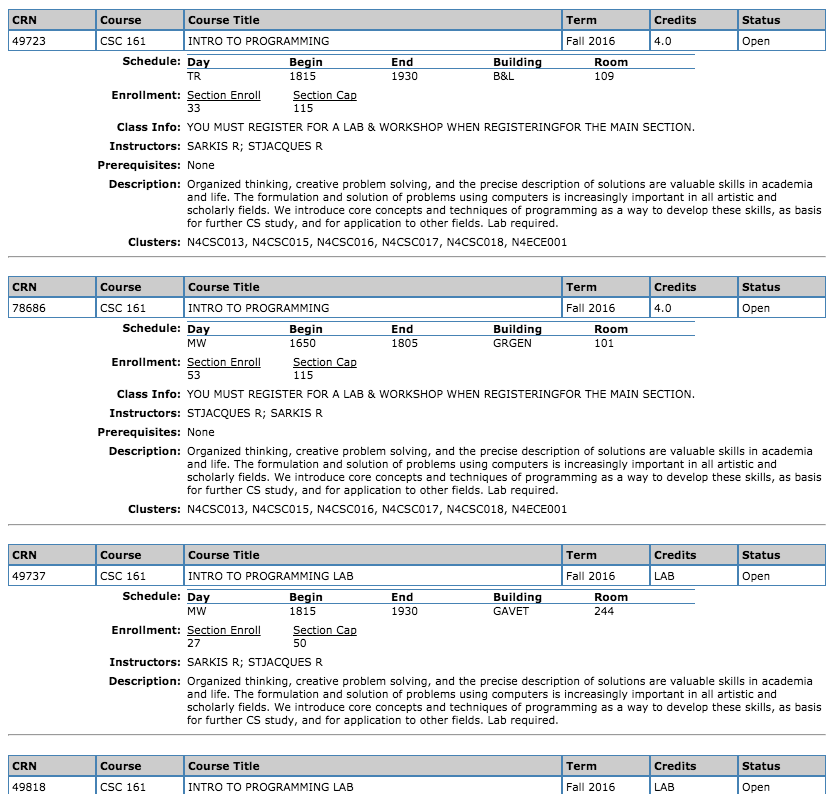
\includegraphics[width=1.00\textwidth]{images/cdcs/sections}
      }
      \caption{Ungrouped sections in CDCS} \label{fig:cdcs-sections}
    \end{subfigure}
    \hspace{15pt}
    \begin{subfigure}[h]{7cm}
      \centering
      \fbox{
        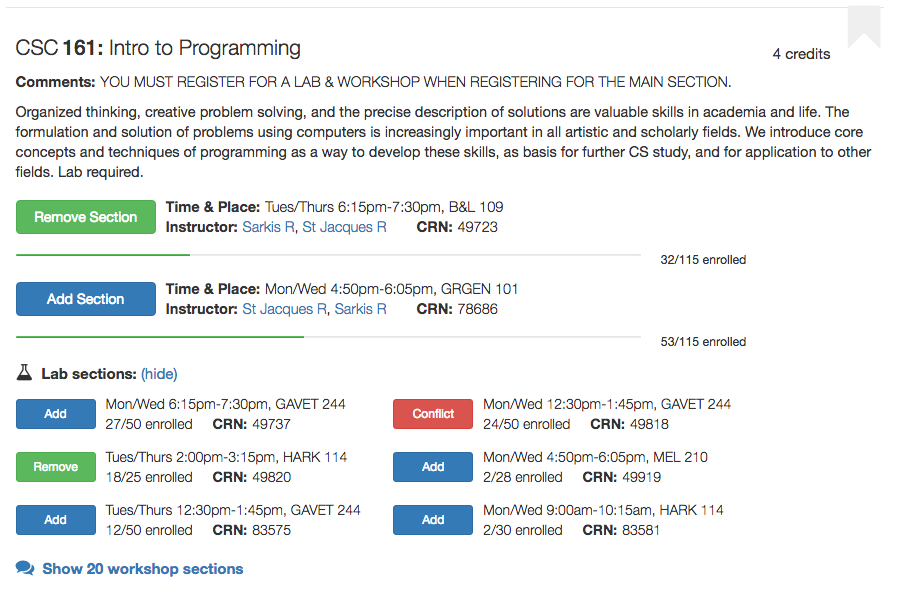
\includegraphics[width=1.00\textwidth]{images/skedge/sections}
      }
      \caption{Grouped sections in Skedge} \label{fig:sk-sections}
    \end{subfigure}
  \end{tabular}
  \caption{Section and subsection presentation in CDCS and Skedge}
\end{figure}


\subsection{Course reference}

\emph{Course mentions} will often appear in the prequisites, crosslists, comments, or description fields of a course (e.g. ``\textbf{Prerequisites:} CSC 171 or equivalent; MTH 150 is REQUIRED''). Users frequently want to find out more information about mentioned courses (frequency shown in Chapter 4). In CDCS, because course mentions are displayed as ordinary plaintext, users have to scroll back up, make a search for \emph{that} course, and lose their current search context as a result.

Skedge solves this by hyperlinking each course mention to a search query for its respective course, in the style of Wikipedia. Moreover, it protects users from a context-switch by displaying a lightweight popover with that course's information when the user hovers their cursor over the course mention (see Figure \ref{fig:sk-hover}).

\begin{figure}[ht]
  \centering
  \vspace{10pt}
  \fbox{
    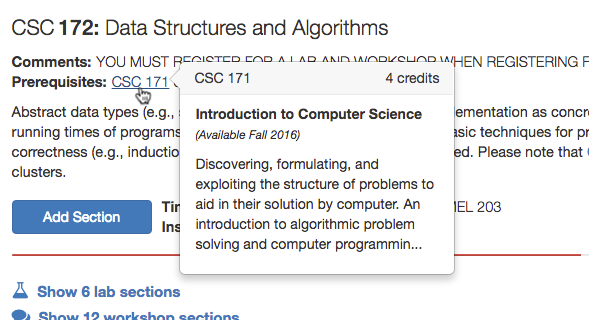
\includegraphics[width=8cm]{images/skedge/hover}
  }
  \caption{Hoverable and clickable course mention in the \emph{Prerequisites} field of a course} \label{fig:sk-hover}
\end{figure}

\subsection{Multiple schedule support}

- Old CDCS+betterCDCS system can't keep track of this, have conflicts when adding stuff
- Multiple schedules per semester (for different schedule possibilities)

\subsection{Exporting}

to Google Calendar, {\tt .ics}, image

- Mobile sync support
- Export gcal is currently broken
- Security: BetterCDCS ``sign in'' sends netID in PLAINTEXT over http(!!!)

\section{Search friendliness}

Of course, the most important usability concern for a course explorer/scheduler is being able to effectively \emph{find courses}.

In this section, I will present the \emph{Skedge DSQL}, a domain-specific query language that is based on natural language. Next, I will demonstrate how Skedge leverages the DSQL to handle the three search criteria students have for finding courses better than CDCS does.

\subsection{Natural language search}

In the spirit of this chapter's theme, Skedge's search method was, again, primarily designed as a reaction to CDCS's. CDCS's search method is a 15-field form (see Figure \ref{fig:cdcs-search}), of which I only found myself regularly using two (one of them being the \emph{required} ``Year/Term'' field). This prompted me to closely examine the fields to a) determine redundancies between them and b) find how to make some of the valuable filter fields more usable. From this came Skedge's unified, natural language based search method, which I call the \emph{Skedge Domain-Specific Query Language (Skedge DSQL)}. Figure \ref{fig:sk-search} is a list of example possible searches shown to users as they type.

\begin{figure}[ht]
  \centering
  \vspace{5pt}
  \begin{tabular}{c c}
    \begin{subfigure}[w]{4.5cm}
      \centering
      \fbox{
        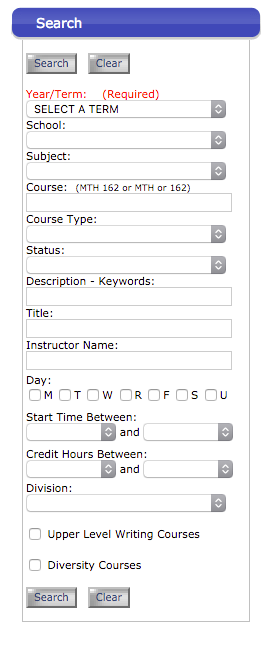
\includegraphics[width=3.3cm]{images/cdcs/search}
      }
      \caption{Form-based search in CDCS} \label{fig:cdcs-search}
    \end{subfigure}
    \hspace{5pt}
    \begin{subfigure}[w]{8.5cm}
      \centering
      \fbox{
        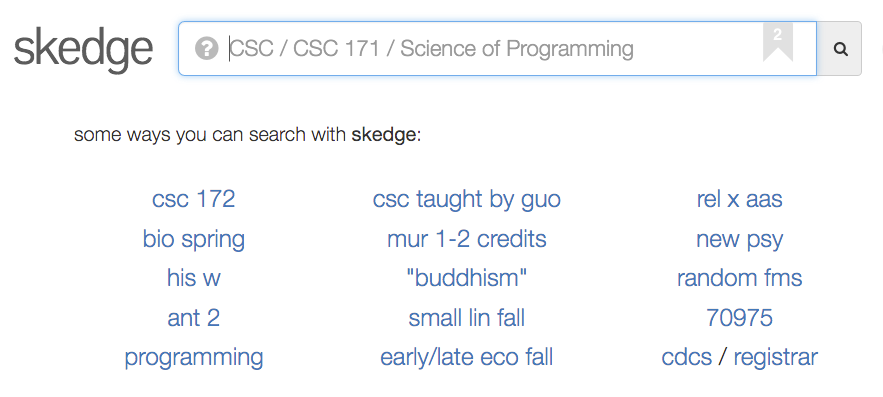
\includegraphics[width=1.00\textwidth]{images/skedge/search}
      }
      \caption{Examples of the Skedge DSQL} \label{fig:sk-search}
    \end{subfigure}
  \end{tabular}
  \caption{Two philosophies of search method}
\end{figure}

\begin{figure}[ht]
  \centering
  \vspace{10pt}
  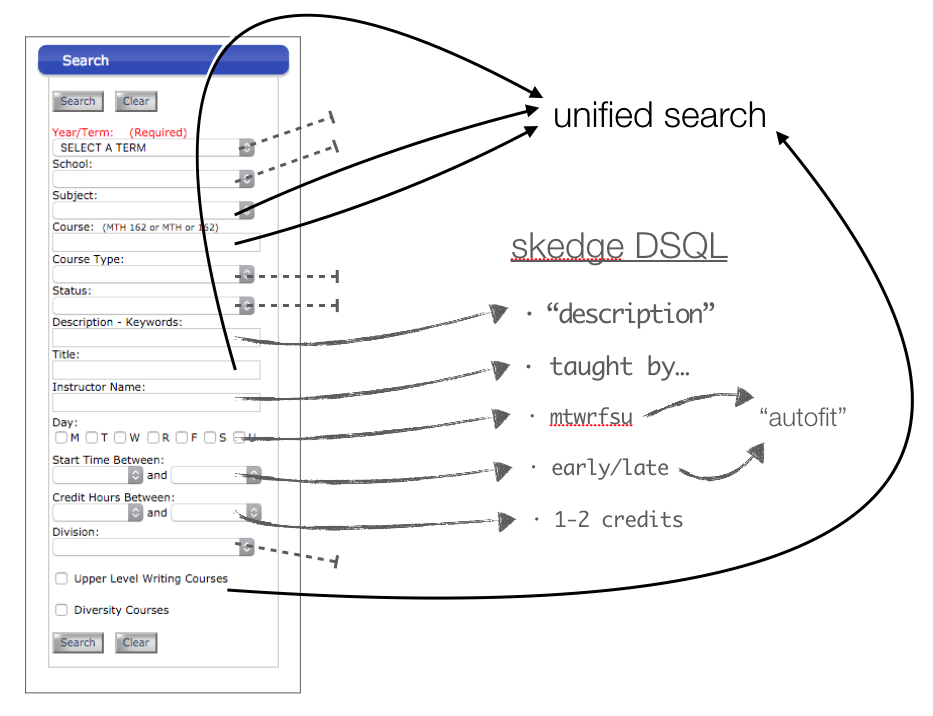
\includegraphics[width=12cm]{images/search-mapping}
  \caption{Mapping from CDCS's form-based search to the Skedge DSQL} \label{fig:search-mapping}
\end{figure}

Figure \ref{fig:search-mapping} is a mapping of each CDCS field to an element of the Skedge DSQL.

  \subsubsection{Advantages of the DSQL}

  - 15 fields reduced to 1

  vs form entry:
  - Faster
  - More intuitive
  - More easily extendable

  - Class size sort

  \subsubsection{Disadvantages of the DSQL}
  grammar ambiguities (can be solved with a `did you mean')

    fall of the roman empire thing

  Having to know the DSL, 

  DSL can be self-taught by the search system being multi-purposed. Used by other links (instructors, course references) around the site. Chapter 4.


\subsection{Course selection criteria}

I have identified \emph{three} use-cases for course searching (the existence of and distinction between these cases will be demonstrated with collected usage data in Chapter 4). The three cases are \textbf{requirements}, \textbf{electives}, and \textbf{peer recommendations}. The Skedge DSL and other application features offer substantial improvements over CDCS for each of these cases. 

  \subsubsection{Requirements}

  These are courses that are required for a student to complete their degree, and are typically searched for directly. The functionality required here is simple and is mostly satisfied by CDCS, but Skedge offers the following improvements to the process:

  \begin{enumerate}
    \item \emph{Crosslisted courses:} For students with more than one major and/or minor, searching for courses that are crosslisted between departments can be valuable in reducing their requirement load. This search filter is unsupported by CDCS, and is supported by Skedge using the operator ``{\tt x}'' (e.g. ``{\tt csc x ece}'' for courses listed under both Computer Science and Electrical \& Computer Engineering departments).

    \item \emph{Clusters:} Skedge already stores a users' previously taken courses, so it can intelligently suggest either already-completed clusters or courses that would complete clusters that are missing one or two courses. For students with many degree requirements already, this could greatly reduce time spent navigating the University's Cluster Search Engine (for which I also have a long list of grievances, but that lies outside the scope of this paper.)\footnote{This feature is under development and is not currently live. It was, incidentally, requested by a Skedge user.}

    \item \emph{CRN:} Surprisingly, search by Course Reference Number is unsupported by CDCS. It is supported by Skedge by just searching the 5-digit number.
  \end{enumerate}

  \subsubsection{Electives}

  Elective courses can be courses within a user's major. Here, Skedge offers search, filter, and sorting features that substantially aid users in browsing courses that they might want to take.

  \begin{enumerate}

    \item ``New'' courses
    \item ``Autofit'' search\footnote{This feature is under development and is not currently live.}
    \item search by instructor
    \item Random
    \item Sorts

  \end{enumerate}

  \subsubsection{Peer Recommendations}

  CDCS currently has no support at all for peer course recommendation, a highly undervalued resource for course finding. Skedge implements peer recomendations through ``Skedge Social,'' a system detailed in the next section.

%%%

\section{``Skedge Social''}

The question ``what are you taking this semester?'' is certainly the most common smalltalk phrase uttered on campus within the first few weeks of the semester. Besides the pure motivation  and it is not unreasonable to assume that students want to take classes that their friends are taking.

\begin{itemize}
  \item ``What are my friends taking?''
  \item ``What do my friends recommend?''
\end{itemize}

\subsection{The issue}

  \subsubsection{Static image vs. live site}

  - Edits don’t update
  - Referencing courses

  \subsubsection{Finding common courses}

  - requires your friends to share their schedules on FB publicly and you to see their post


%%%%%%%%%%%%%%


  - is schedule-first, not search-first
  - typically only occurs for the current semester

%figure

\subsection{Skedge's solution}

% Walkthru

  \subsubsection{Friends' course enrollments}

  Mini-feed

  \subsubsection{Friends' course likes}

  \subsubsection{Likes \& enrollments embedded in results}

  \subsubsection{Personal schedule synchronization}

  \subsubsection{Privacy}

  \subsubsection{Notifications}

  %figs of the 2 types